\documentclass[
	10pt,								% globale Schriftgröße
	parskip=half-,						% setzt Absatzabstand hoch
	paper=a4,							% Format
	english,ngerman,					% lädt Sprachpakete
	]{scrartcl}							% Dokumentenklasse

% //////////////////// Pakete laden ////////////////////
\usepackage[fleqn]{amsmath}
\usepackage[fleqn]{mathtools}
\usepackage{amssymb}			% mathematische symbole, für \ceckmarks
\usepackage{amsthm}				% für proof
\usepackage{mathrsfs}			% für \mathscr
\usepackage{latexsym}
\usepackage{marvosym}				% für Lightning

\usepackage{fontspec} 			% funktioniert nur mit den neueren Compilern z.B. XeLaTeX
\usepackage{microtype}			% für bessere Worttrennung
\usepackage[ngerman]{babel} 	% Spracheinstellung
\usepackage{lmodern}			% verändert verwendete Schriftart, damit sie weniger pixelig ist

\usepackage{verbatim}
\usepackage{listings}			% Für Quellcode

\usepackage{graphicx}
\usepackage{tabularx}			% für Tabellen mit gleicher Spaltenbreite und automatischen Umbrüchen
\usepackage{fullpage}
\usepackage{multirow}			% für multirow in tabulars
\usepackage{rotate}
\usepackage[cmyk,table]{xcolor} % um Farben zu benutzen, kann mehr als das Paket color
\usepackage[					% Verlinkungen
	colorlinks,					% farbige Schrift, statt farbiger Rahmen
	linktocpage,				% verlinkt im Abb.Verzeichnis Seitenzahl statt Bildunterschrift
	linkcolor=blue				% setzt Farbe der Links auf blau
	]{hyperref}					% nur für digitale Anwendungen, url = "http://www.example.com"
\usepackage{url}				% für Webadressen wie e-mail usw.: "\url{http://www.example.com}"

\usepackage{enumerate}			% für versch. Aufzählungezeichen wie z.B. a)
\usepackage{xspace}				% folgt ein Leerzeichen nach einem \Befehl, wird es nicht verschluckt.
\usepackage{cancel}				% für das Durchstreichen u.a. in Matheformeln mit \cancel
\usepackage{float}              % zum Forcieren der Position von figure-Umgebungen

% zum Zeichnen (u.a. von Graphen)
\usepackage{fp}
\usepackage{tikz}
\usetikzlibrary{tikzmark}			% für \tikzmark{toRemember}
\usetikzlibrary{positioning}	% verbesserte Positionierung der Knoten
\usetikzlibrary{automata}		% für Automaten (GTI)
\usetikzlibrary{arrows}
\usetikzlibrary{shapes}
\usetikzlibrary{decorations.pathmorphing}
\usetikzlibrary{decorations.pathreplacing}
\usetikzlibrary{decorations.shapes}
\usetikzlibrary{decorations.text}

% //////////////////// Syntaxhighlighting ////////////////////
\lstloadlanguages{Python, Haskell, [LaTeX]TeX, Java}
\lstset{
   basicstyle=\footnotesize\ttfamily,	% \scriptsize the size of the fonts that are used for the code
   backgroundcolor = \color{bgcolour},	% legt Farbe der Box fest
   breakatwhitespace=false,	% sets if automatic breaks should only happen at whitespace
   breaklines=true,			% sets automatic line breaking
   captionpos=t,				% sets the caption-position to bottom, t for top
   commentstyle=\color{codeblue}\ttfamily,% comment style
   frame=single,				% adds a frame around the code
   keepspaces=true,			% keeps spaces in text, useful for keeping indentation
							% of code (possibly needs columns=flexible)
   keywordstyle=\bfseries\ttfamily\color{codepurple},% keyword style
   numbers=left,				% where to put the line-numbers;
   							% possible values are (none, left, right)
   numberstyle=\tiny\color{codegreen},	% the style that is used for the line-numbers
   numbersep=5pt,			% how far the line-numbers are from the code
   stepnumber=1,				% nummeriert nur jede i-te Zeile
   showspaces=false,			% show spaces everywhere adding particular underscores;
							% it overrides 'showstringspaces'
   showstringspaces=false,	% underline spaces within strings only
   showtabs=false,			% show tabs within strings adding particular underscores
   flexiblecolumns=false,
   tabsize=1,				% the step between two line-numbers. If 1: each line will be numbered
   stringstyle=\color{orange}\ttfamily,	% string literal style
   numberblanklines=false,				% leere Zeilen werden nicht mitnummeriert
   xleftmargin=1.2em,					% Abstand zum linken Layoutrand
   xrightmargin=0.4em,					% Abstand zum rechten Layoutrand
   aboveskip=2ex, 
}

\lstdefinestyle{py}{
   language=Python,
}
\lstdefinestyle{hs}{
   language=Haskell,
}
\lstdefinestyle{tex}{
	language=[LaTeX]TeX,
	escapeinside={\%*}{*)},     % if you want to add LaTeX within your code
	texcsstyle=*\bfseries\color{blue},% hervorhebung der tex-Schlüsselwörter
	morekeywords={*,$,\{,\},\[,\],lstinputlisting,includegraphics,
	rowcolor,columncolor,listoffigures,lstlistoflistings,
	subsection,subsubsection,textcolor,tableofcontents,colorbox,
	fcolorbox,definecolor,cellcolor,url,linktocpage,subtitle,
	subject,maketitle,usetikzlibrary,node,path,addbibresource,
	printbibliography},% if you want to add more keywords to the set
     numbers=none,
     numbersep=0pt,
     xleftmargin=0.4em,
}

\lstdefinestyle{java}{
	language=Java,
	extendedchars=true,		% lets you use non-ASCII characters;
   						% for 8-bits encodings only, does not work with UTF-8
}

\lstdefinelanguage[x64]{Assembler}     % add a "x64" dialect of Assembler
   [x86masm]{Assembler} % based on the "x86masm" dialect
   % with these extra keywords:
   {morekeywords={CDQE,CQO,CMPSQ,CMPXCHG16B,JRCXZ,LODSQ,MOVSXD, %
                  POPFQ,PUSHFQ,SCASQ,STOSQ,IRETQ,RDTSCP,SWAPGS, %
                  rax,rdx,rcx,rbx,rsi,rdi,rsp,rbp, %
                  r8,r8d,r8w,r8b,r9,r9d,r9w,r9b}
}					% for 8-bits encodings only, does not work with UTF-8

\lstdefinestyle{c}{
	language=c,
	extendedchars=true,		% for 8-bits encodings only, does not work with UTF-8
}

% //////////////////// eigene Kommandos ////////////////////
\newcommand\FU{Freie Universität Berlin\xspace}% benötigt package xspace
\newcommand\gdw{g.\,d.\,w.\xspace}
\newcommand\oBdA{o.\,B.\,d.\,A.\xspace}
\newcommand{\Eu}{\texteuro}
\newcommand\N{\mathbb{N}\xspace}
\newcommand\Q{\mathbb{Q}\xspace}
\newcommand\R{\mathbb{R}\xspace}
\newcommand\Z{\mathbb{Z}\xspace}
\newcommand\ohneNull{\ensuremath{\backslash\lbrace 0\rbrace}}% \{0}
\let\dhALT\dh	% Schreibt Befehl \dh in \dhALT um
\renewcommand\dh{d.\,h.\xspace}	%renew überschreibt command \dh
\newcommand\Bolt{\;\text{\LARGE\raisebox{-0.3em}{\Lightning}\normalsize}\xspace}% Blitz
\newcommand\zz{\ensuremath{\raisebox{+0.25ex}{Z}% zu zeigen
			\kern-0.4em\raisebox{-0.25ex}{Z}%
			\;\xspace}}
\newcommand{\from}{\ensuremath{\colon}}
\newcommand{\floor}[1]{\lfloor{#1}\rfloor}
\newcommand{\ceil}[1]{\lceil{#1}\rceil}
 \renewcommand{\L}{\ensuremath{\mathcal{L}}\xspace}
 \renewcommand{\P}{\ensuremath{\mathcal{P}}\xspace}
 \newcommand{\NL}{\ensuremath{\mathcal{N}\kern-0.2em\mathcal{L}}\xspace}
 \newcommand{\NP}{\ensuremath{\mathcal{NP}}\xspace}

% //////////////////// Mathefunktionen ////////////////////
\DeclareMathOperator{\Landau}{\mathcal{O}}
\DeclareMathOperator{\True}{True}
\DeclareMathOperator{\False}{False}

% //////////////////// eigene Theoreme ////////////////////
\newtheorem{theorem}{Satz}
\newtheorem{corollary}[theorem]{Folgerung}
\newtheorem{lemma}[theorem]{Lemma}
\newtheorem{observation}[theorem]{Beobachtung}
\newtheorem{definition}[theorem]{Definition}
\newtheorem{Literatur}[theorem]{Literatur}
% konfiguriert proof
\makeatletter
\newenvironment{Proof}[1][\proofname]{\par
  \pushQED{\qed}%
  \normalfont \topsep6\p@\@plus6\p@\relax
  \trivlist
  \item[\hskip\labelsep
%         \itshape
        \bfseries
    #1\@addpunct{.}]\ignorespaces
}{%
  \popQED\endtrivlist\@endpefalse
}
\makeatother

% //////////////////// eigene Farben ////////////////////
\let\definecolor=\xdefinecolor
\definecolor{FUgreen}{RGB}{153,204,0}
\definecolor{FUblue}{RGB}{0,51,102}

\definecolor{middlegray}{rgb}{0.5,0.5,0.5}
\definecolor{lightgray}{rgb}{0.8,0.8,0.8}
\definecolor{orange}{rgb}{0.8,0.3,0.3}
\definecolor{azur}{rgb}{0,0.7,1}
\definecolor{yac}{rgb}{0.6,0.6,0.1}
\definecolor{Pink}{rgb}{1,0,0.6}

\definecolor{bgcolour}{rgb}{0.97,0.97,0.97}
\definecolor{codegreen}{rgb}{0,0.6,0}
\definecolor{codegray}{rgb}{0.35,0.35,0.35}
\definecolor{codepurple}{rgb}{0.58,0,0.82}
\definecolor{codeblue}{rgb}{0.4,0.5,1}

% //////////////////// eigene Settings ////////////////////

\textheight = 230mm		% Höhe des Satzspiegels / Layouts
\footskip = 10ex			% Abstand zw. Fußzeile und Grundlinie letzter Textzeile
\parindent 0pt			% verhindert Einrückung der 1. Zeile eines Absatzes
\setkomafont{sectioning}{\rmfamily\bfseries}% setzt Ü-Schriften in Serifen, {disposition}											% bindet Header ein (WICHTIG)
\usepackage{graphicx}
\usepackage{amsmath}
\usepackage{amssymb}
\usepackage{fancyvrb}

\newcommand{\dozent}{Prof. Dr. Margarita Esponda}					% <-- Names des Dozenten eintragen
\newcommand{\tutor}{Lilli Walter}						% <-- Name eurer Tutoriun eintragen
\newcommand{\tutoriumNo}{6}				% <-- Nummer im KVV nachschauen
\newcommand{\projectNo}{5}									% <-- Nummer des Übungszettels
\newcommand{\veranstaltung}{Nichtsequentielle Programmierung}	% <-- Name der Lehrveranstaltung eintragen
\newcommand{\semester}{SoeSe 2017}						% <-- z.B. SoSo 17, WiSe 17/18
\newcommand{\studenten}{Boyan Hristov, Sergelen Gongor}			% <-- Hier eure Namen eintragen
% /////////////////////// BEGIN DOKUMENT /////////////////////////


\begin{document}
% /////////////////////// BEGIN TITLEPAGE /////////////////////////
\begin{titlepage}
	\subject{\dozent}
	\title{\veranstaltung, \semester}
	\subtitle{\Large Übungsblatt \projectNo\\ \large\vspace{1ex} TutorIn: \tutor\\ Tutorium \tutoriumNo}
	\author{\studenten}
	\date{\normalsize \today}
\end{titlepage}

\maketitle								% Erstellt das Titelblatt
\vspace*{-10cm}							% rückt Logo an den oberen Seitenrand
\makebox[\dimexpr\textwidth+1cm][r]{	%rechtsbündig und geht rechts 1cm über Layout hinaus
	
\includegraphics[width=0.4\textwidth]{src/fu_logo} % fügt FU-Logo ein
}
% /////////////////////// END TITLEPAGE /////////////////////////

\vspace{7cm}							% Abstand
\rule{\linewidth}{0.8pt}				% horizontale Linie										% erstellt die Titelseite


Link zum Git Repository: \url{https://github.com/BoyanH/FU-Berlin-ALP4/tree/master/Solutions/Homework5}

% /////////////////////// Aufgabe 1 /////////////////////////

\section*{Aufgabe 1}

\begin{enumerate}

\item $\square A \land \lozenge B \Rightarrow \lozenge (A \land B)$

\begin{align*}
	& \square A \land \lozenge B \\
	\Leftrightarrow  & \forall k \geq i: A \land \exists j \geq i: B \\
	\Leftrightarrow & \exists j \geq i: A \land B \tag{Da A für alle k $\geq$ i wahr ist, dann auch für j} \\
	\Leftrightarrow & \lozenge (A \land B) 
\end{align*}

\item $\square (A \lor B) \Rightarrow ( \square A \lor \lozenge B)$

\begin{align*}
	& \square (A \lor B) \\ \\
	\Leftrightarrow & \forall k \geq i: A \lor B \\
	 & \text{Sei Z die Menge aller } p \geq i \text{ mit A wahr in } S_p 
	 \text{, dann gilt} \\
	 & \forall z \in Z: A \land \forall q \geq i, q \not\in Z: B \\
	 \Rightarrow & \square A \lor \square B \lor \lozenge A \lor \lozenge B \\
	 \Rightarrow & (\square A \lor \lozenge B)
\end{align*}

Die Formale Begründung war schwierig und uns reichte die formale Notation nicht aus, aber informal: \\
Das linke Teil der Implikation sagt, dass in jedem Zustand gilt mindestens eine von den beiden A und B. Dann muss entweder eine von den beiden immer gelten, oder wenn es mindestens ein Zustand gibt, wo das eine nicht gilt, muss das andere in diesem Zustand gelten. D.h. wenn A nicht immer wahr ist, must B irgendwann wahr sein und umgekehrt. \\ \\
Da aber $\square B \Rightarrow \lozenge B$, oder wenn B immer gilt, dann gilt irgendwann B, kann man aus dem linken Teil der Implikation den rechten ableiten, oder anders gesagt, wenn das linke wahr ist, ist das rechte Teil auch immer wahr. \\ \\

\item $\lozenge A \land \lozenge B \Rightarrow \lozenge (A \land B)$

Diese Aussage ist falsch. Gegenbeispiel:

\begin{align*}
	& \text{Sei A wahr in $S_j$ bis $S_{j+2}$ und B wahr von $S_{j+4}$ bis $S_{j+6}$, dann gilt} \lozenge A \land \lozenge B \text{ aber nicht } \lozenge(A \land B)
\end{align*}

Informal: Das linke Teil sagt, dass jede Aussage in mindestens einem beliebigen Zustand wahr ist, aber nicht das beide Aussagen in einem beliebigen Zustand wahr sind, was das rechte Teil ist. In der Vorlesung wurde $\square \lozenge A \land \square \lozenge B \not\Rightarrow \lozenge (A \land B)$ gezeigt, was eigentlich eine Obermenge von dieser Aufgabe ist. Da haben wir gesehen, dass auch wenn die zwei Aussagen ständig wieder wahr werden, gibt es keine Garantie, dass diese irgendwann zusammen beide gelten werden.

\end{enumerate}


\section*{Aufgabe 2}

\begin{enumerate}

\item n=4, k=2 \\

Die erste zwei Threads laufen bis $p_8$ nach einander. D.h. $ count=0 \land D = 0$. Dan laufen zwei weitere Threads nach einander bis $p_7$. D.h. $count=-2$ und die letzte beide Threads warten auf D. Danach laufen die erste zwei Threads bis $p_1$. Das erste Thread setzt $count = count + 1 = -2 + 1 = -1 \leq 0$ und released deswegen D. Dann wird das 2 Thread, das sich im CS befindet bis $p_1$ ausgeführt, setzt dabei $count = count+1 = -1 + 1 = 0 \leq 0 \Rightarrow$ releaset D wieder. Damit haben wir $D=2$ erreicht, ein unerlaubtes Zustand. 

\item n=3, k=2 \\

$T_1$ und $T_2$ laufen bis $p_8$, damit ist count = 0, D = 0. $T_3$ läuft bis $p_7$ und wartet auf D, count = -1. $T_1$ läuft bis $p_7$, setzt dabei count = 0 in $p_10$ und wieder count = -1 in $p_3$, deswegen geht er in die if-Anweisung. D wird von $T_1$ dabei release-t und es gilt jetzt D = 1. $T_2$ macht das selbe, da count = -1 setzt dieses count = 0 in $p_10$ und wieder $count=3$ in $p_3$. Dabei release-t er aber auch D, da count = 0 war als er durchgelaufen ist, deswegen ist jetzt D = 2, ein unerlaubtes Zustand.

Das kann passieren nur wenn $T_1$ und $T_2$ in $p_6$ oder $p_7$ lang genug hängen bleiben, wenn der Scheduler diese nicht laufen lässt, diese aber warten seit dem $T_1$ $p_12$ ausgeführt hat nicht mehr auf acquire(D)!!!

\end{enumerate}

\section*{Aufgabe 3}

Unsere Lösung funktioniert mit den Invarianten:

\begin{enumerate}

\item Nur 3 Threads werden durch den Barrier auf einmal durchgelassen (durch Java garantiert), maximal 3 warten

Formal: barrier.getParties() = 3 $\land$ barrier.getNumberWaiting() $\geq 3$ \\

\item Nur 2 Wasserstoff und 1 Sauerstoff Atome können gleichzeitig an der Barriere warten. Wird durch den Semaphoren garantiert.
 
Formal: Hydrogen.hydrogens.availablePermits() $\geq 2$ $\land$ Oxygen.oxygens.availablePermits() $\geq 1$

\end{enumerate}

\begin{lstlisting}[style=java]

package fu.alp4;

import java.util.concurrent.CyclicBarrier;

public class Main {

    public static void main(String[] args) {
        final CyclicBarrier barrier = new CyclicBarrier(3);

        while (true) {
            double random = Math.random();

            if (random > 0.4) {
                new Hydrogen(barrier).start();
            } else {
                new Oxygen(barrier).start();
            }

            Nap.randomNap(1000, 3000);
        }

    }
}

\end{lstlisting}

\begin{lstlisting}[style=java]

package fu.alp4;

import java.util.concurrent.BrokenBarrierException;
import java.util.concurrent.CyclicBarrier;
import java.util.concurrent.locks.Lock;
import java.util.concurrent.locks.ReentrantLock;

public abstract class BarrierReleaseHandler extends Nap {

    static int waterMolecules = 0;
    private Lock incrementLock = new ReentrantLock();
    private CyclicBarrier barrier;

    public BarrierReleaseHandler(CyclicBarrier bondingBarrier) {
        this.barrier = bondingBarrier;
    }

    protected void awaitBarrier() throws BrokenBarrierException, InterruptedException {
        int turn = this.barrier.await();

        /**
         * The first thread to arrive at the barrier will be the one to create the water molecule.
         * Method created to share functionality between Hydrogen and Oxygen classes
         */

        if (turn == 0) {
            incrementLock.lock();
            BarrierReleaseHandler.waterMolecules++;
            System.out.printf("A new water molecule was created! Water molecules: %d\n", BarrierReleaseHandler.waterMolecules);
            incrementLock.unlock();
        }
    }
}

\end{lstlisting}


\begin{lstlisting}[style=java]

package fu.alp4;

import java.util.concurrent.BrokenBarrierException;
import java.util.concurrent.CyclicBarrier;
import java.util.concurrent.Semaphore;

public class Hydrogen extends BarrierReleaseHandler {

    static final Semaphore hydrogens = new Semaphore(2);

    public Hydrogen (CyclicBarrier bondingBarrier) {
        super(bondingBarrier);
    }

    public void run() {

        System.out.println("Hydrogen atom appeared from nowhere!");
        Hydrogen.randomNap(2000, 5000);
        System.out.println("Hydrogen atom wants to bond!");
        try {
            /**
             * allow only up to 2 hydrogens to wait at the barrier
             */
            this.hydrogens.acquire();
            System.out.println("Hydrogen atom is ready to bond, waiting on the barrier!");
        } catch (InterruptedException e) {
            e.printStackTrace();
            return;
        }

        try {
            this.awaitBarrier();
        } catch (InterruptedException e) {
            e.printStackTrace();
        } catch (BrokenBarrierException e) {
            e.printStackTrace();
        }

        // release back the available spots after molecule bonding
        hydrogens.release();
    }
}

\end{lstlisting}

\begin{lstlisting}[style=java]

package fu.alp4;

import java.util.concurrent.BrokenBarrierException;
import java.util.concurrent.CyclicBarrier;
import java.util.concurrent.Semaphore;

public class Oxygen extends BarrierReleaseHandler {

    static final Semaphore oxygens = new Semaphore(1);
    private CyclicBarrier barrier;

    public Oxygen(CyclicBarrier bondingBarrier) {
        super(bondingBarrier);
    }

    public void run() {

        System.out.println("Oxygen atom appeared from nowhere!");
        Hydrogen.randomNap(2000, 5000);
        System.out.println("Oxygen atom wants to bond!");
        try {
            this.oxygens.acquire();
            System.out.println("Oxygen atom is ready to bond, waiting on the barrier!");
        } catch (InterruptedException e) {
            e.printStackTrace();
            return;
        }

        try {
            this.awaitBarrier();
        } catch (InterruptedException e) {
            e.printStackTrace();
        } catch (BrokenBarrierException e) {
            e.printStackTrace();
        }

        oxygens.release();
    }
}


\end{lstlisting}

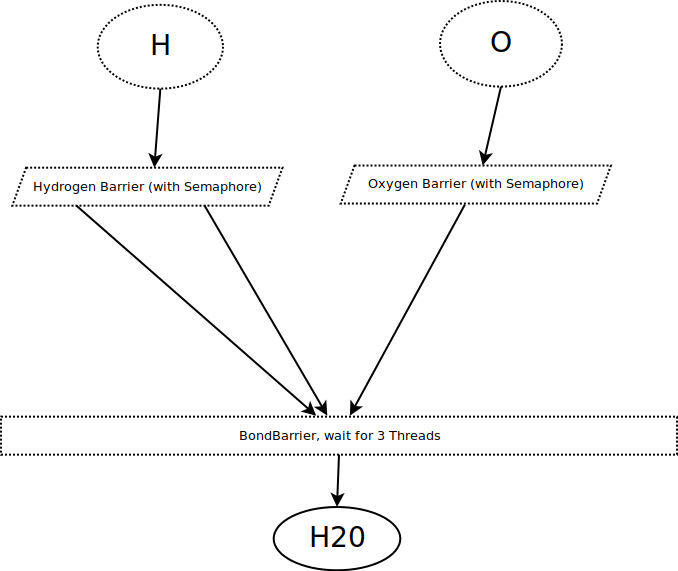
\includegraphics[width=\textwidth]{./exercise3/Diagram1.png}

\section*{Aufgabe 4}

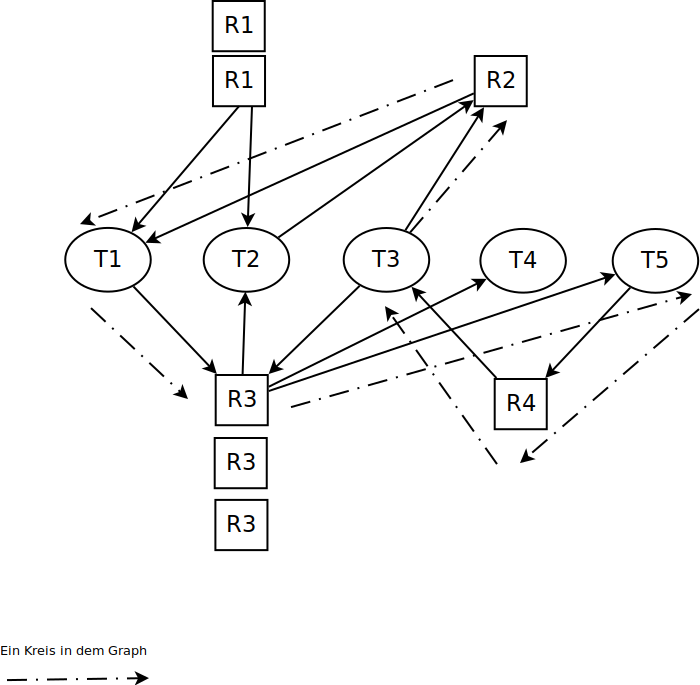
\includegraphics[width=\textwidth]{./exercise4.png}

Ein Kreis haben wir auf dem Graphen dargestellt, es existiert aber noch ein weiteres und nämlich $T_2 \rightarrow R_2 \rightarrow T_1 \rightarrow R_3 \rightarrow T_2$. 

\begin{enumerate}

\item Der Graph befindet sich in einem von Deadlock gefährdeten Zustand, da es Zyklen in dem Graph gibt

\item Da es keine Kreis / Zyklus / Schleife zu finden ist, wo nur einzelne Resourcen ($R_i = 1 \forall i \in R$), können wir nicht mit Sicherheit sagen, dass es Deadlock gibt. Nach unserer Beobachtung haben wir keine gefunden.

\end{enumerate}

\section*{Aufgabe 5}

Da es maximal n+m Resourcen angefordert werden müssen, heißt es auch in dem Fall, dass ein Thread extrem Resourcenaufwändig ist und n-1 Resourcen schon genommen hat und n allgemein braucht, aber nicht das letzte sich geholt hat damit es terminiert und die Resourcen wieder freigibt, gibt es immer noch m-2 Threads die nur eine Resource brauchen und frei funktionieren können.


Wie wir schon kennen, ist es aber am gefährlichsten wenn alle Threads ungefähr gleich viele Resourcen brauchen. Sei k diese Anzahl, dann ist die gefährlichste Situation, wenn jeder Thread k-1 Resourcen sich geholt hat, aber das letzte noch nicht und terminiert deswegen nicht, gibt auch keine Resourcen noch frei. In diesem Fall sind das $\floor{\frac{(n+m -1)}{m}}$ Resourcen pro Prozess. Also jedes Prozess nimmt initial $\floor{\frac{(n+m -1)}{m} - 1 } = \floor{\frac{n}{m} + 1 - \frac{1}{m} }$ Resourcen. Da das keine ganze Zahl (wegen $\frac{1}{m}$) ist bleibt immer ein (genau 1 wegen $m\frac{1}{m}$) Resource frei / bzw. ein Thread braucht wenigere Resourcen und kann terminieren und die Resourcen wieder frei lassen. 

% /////////////////////// END DOKUMENT /////////////////////////
\end{document}